\documentclass[12pt,a4paper,twoside,openright]{book}

\usepackage[italian]{babel}
\usepackage{style/isi-lt}
\usepackage{cite}
\usepackage{svg}
\usepackage{calc}

\definecolor{dkgreen}{rgb}{0,0.6,0}
\definecolor{gray}{rgb}{0.5,0.5,0.5}
\definecolor{mauve}{rgb}{0.58,0,0.82}

\lstset{
  frame=single,
  captionpos=b,
  language=Java,
  aboveskip=3mm,
  belowskip=3mm,
  showstringspaces=false,
  columns=flexible,
  basicstyle={\small\ttfamily},
  numbers=none,
  numberstyle=\tiny\color{gray},
  keywordstyle=\color{blue},
  commentstyle=\color{dkgreen},
  stringstyle=\color{mauve},
  breaklines=true,
  breakatwhitespace=true,
  tabsize=3
}

%--------------------------------------------------------------------
%---------------------- INFORMAZIONI SULLA TESI ---------------------
%--------------------------------------------------------------------

\universita{Alma Mater Studiorum -- Università di Bologna}
\campus{Campus di Cesena}
\dipartimento{Dipartimento di Informatica -- Scienza e Ingegneria}
\cdl{Corso di Laurea in Ingegneria e Scienze Informatiche}

% \titolo{Qui il titolo\\della\\tesi}
\titolo{Sviluppo di backend \\per il linguaggio Protelis \\in Kotlin e Java}
\materia{Programmazione ad Oggetti}

\laureando{Filippo Nardini}

\relatore[Prof.]{Danilo Pianini}
\correlatorea[Prof.]{Mirko Viroli}

\annoaccademico{2018 -- 2019}

\dedica{A Coro, mia fonte di ispirazione suprema.}

\makeindex

\begin{document}
\frontmatter

\maketitle
\tableofcontents

% L'ambiente da cui siamo circondati tutti i giorni è pervaso da dispositivi in
grado di effettuare computazioni e comunicare. L'eterogeneità di questi
dispositivi rende difficile sviluppare applicazioni distribuite resilienti e
affidabili utilizzando le tecniche dell'ingegneria del software classica. La
programmazione aggregata si propone come paradigma di sviluppo che fornisce
meccanismi di comunicazione flessibili e robusti tra questi dispositivi, in
particolare vengono presi in considerazione il \textit{field calculus} e una sua
implementazione pratica: Protelis, un linguaggio di programmazione che supporta
tale paradigma di programmazione.

In questo lavoro vengono analizzate le caratteristiche di Protelis, in
particolare la sua architettura e i suoi livelli di astrazione. In seguito
vengono modellati nuovi concetti, per la realizzazione di un modello ad oggetti
riusabile, che possa essere un potenziale punto di partenza per
l'implementazione di un'infrastruttura facilmente estendibile, riusabile, e
manutenibile. A supporto della flessibilità del modello, sono presentate tre
realizzazioni dell'architettura descritta, che eseguono lo stesso programma
aggregato, ma finalizzate a descrivere tre scenari d'uso distinti: la prima
rappresenta un micro-simulatore, che emula un contesto distribuito, ma sfrutta
la memoria condivisa per permettere la comunicazione tra i nodi; la seconda
realizza un'applicazione distribuita utilizzando le socket TCP per comunicare;
la terza si serve di un broker di messaggistica centrale e sfrutta il protocollo
MQTT, un modello publish/subscribe, per la trasmissione dei messaggi. Per
provare l'interoperabilità dell'architettura con i linguaggi eseguiti sulla Java
Virtual Machine, questi tre scenari sono stati implementati sia in Java che in
Kotlin.




% La presente tesi è articolata in tre capitoli.
% Nel primo di questi vengono analizzate le caratteristiche dell'architettura
% dell'infrastruttura di Protelis, i vari livelli di astrazione dei quali sono
% costituite le sue API, la sua interoperabilità con altri linguaggi eseguiti
% sulla Java Virtual Machine, e il suo utilizzo nell'ambito scientifico. Nel
% secondo vengono esaminate le API della sua infrastruttura e le sue
% implementazioni esistenti. In questo capitolo vengono introdotti nuovi concetti
% al modello esistente. L'obiettivo di questi è di fornire un modello ad oggetti
% riusabile, che possa essere un potenziale punto di partenza per
% l'implementazione di un'infrastruttura facilmente estendibile, riusabile, e
% manutenibile. Nel terzo sono presentate tre implementazioni del modello
% sviluppato in uno scenario applicativo reale, per dimostrarne la potenziale
% portabilità.  Al fine di provare l'interoperabilità dell'architettura proposta
% con i linguaggi eseguiti sulla Java Virtual Machine, l'implementazione di
% ciascuno scenario è stato effettuata sia in Java che in Kotlin.


\mainmatter

\pagestyle{fancy}
\fancyhead[LE,RO]{\thepage}
\fancyfoot{}

\chapter{Contesto e motivazioni}
\section{Scenario}
Nell'ambiente in cui viviamo siamo circondati da sempre più entità
computazionali eterogenee tra loro. Device come smartphone, smartwatch, fitness
tracker, display pubblici, droni, insegne digitali, sensori di ogni tipo stanno
sempre più pervadendo il nostro ambiente quotidiano. L'interazione tra questi
dispositivi gioca un ruolo fondamentale in settori emergenti come
Internet-of-Things (IoT), Smart City, reti di sensori o più in generale in
sistemi collettivi adattivi. Quando si parla di sistemi collettivi si deve
tenere in considerazione l'elevato numero di dispositivi diversi di cui essi
sono composti e l'eterogeneità che ne deriva in termini di piattaforme,
tecnologie, paradigmi di programmazione, protocolli di comunicazione,
eccetera. Specifiche come efficienza, organizzazione e la necessità di
coordinare i dispositivi, influenzano pesantemente le scelte di design del
sistema, che può risultare rigido, costoso da manutenere, estendere, ed
eventualmente scalare in dimensione.

Sorge quindi la necessità di un modello di programmazione più ad alto livello,
che consenta di astrarre i dettagli di un sistema e possa occuparsi di tutti i
requisiti non funzionali come le proprietà di auto-organizzazione e
auto-adattività, delegando allo strato sottostante tutte le questioni di più basso livello. Possono essere elencate tre caratteristiche
chiave che questo strato dovrebbe presentare\cite{DBLP:journals/computer/BealPV15
}:
\begin{itemize}
\item i meccanismi di comunicazione dovrebbero essere nascosti e i gli
  sviluppatori non dovrebbero essere tenuti a interagire con essi;
\item la composizione di moduli o sottosistemi dovrebbe essere semplice e
  trasparente;
\item sottosistemi distinti necessitano di meccanismi di coordinazione per
  distinte regioni dello spazio-tempo.
\end{itemize}

\begin{figure}
  \centering
  \includegraphics[width=\linewidth]{images/streetscene}
  \caption{Lo spazio che ci circonda è denso di oggetti in grado di effettuare
    calcoli e capaci di comunicare. Alcuni di questi sono oggetti
    infrastrutturali, ma la maggior parte sono oggetti personali, in continuo
    movimento. Immagine tratta da \cite{Protelis}.}
  \label{fig:streetscene}
\end{figure}

\section{Aggregate computing}
\label{sec:aggregate-computing}
\begin{figure}
  \subfloat[Programmazione device-centric]{
    \includegraphics[width=\linewidth]{images/distributed-composition}
    \label{fig:device-centric}
  }\hfill
  \subfloat[Programmazione aggregata]{
    \includegraphics[width=\linewidth]{images/aggregate-composition}
    \label{fig:aggregate-computing}
  }
  \caption{Differenze tra programmazione orientata al singolo dispositivo e
    programmazione aggregata. Immagini tratte da \cite{Protelis}.}
\end{figure}
Spesso la modellazione del comportamento collettivo di un sistema interessa più
del singolo dispositivo di cui è composto, ma i linguaggi di programmazione
classici, orientati al singolo dispositivo, forzano lo sviluppatore a porre
l'attenzione sui singoli device e all'interazione tra di
essi. L'\textit{aggregate computing} è un paradigma che si propone di risolvere
le precedenti questioni tramite i seguenti
principi\cite{DBLP:journals/computer/BealPV15}:
\begin{enumerate}
\item il dispositivo programmato è una regione dell'ambiente computazionale e
  prescinde dagli specifici dettagli;
\item il programma è specificato come manipolazione funzionale di strutture dati
  distribuite nello spazio-tempo di interesse;
\item queste manipolazioni sono effettivamente eseguite dai singoli dispositivi
  nella regione, usando meccanismi di coordinazione resilienti e interazioni
  basate sulla prossimità.
\end{enumerate}

Un esempio di utilizzo nel mondo reale potrebbe essere un servizio che,
utilizzando interazioni tra gli smartphone per stimare la densità di popolazione
presente in un area o ad un certo evento, possa fornire indicazioni relative a
zone che possono essere considerate pericolose perché troppo dense e che percorso
seguire eventualmente per disperderle; più in generale, possono essere erogate
indicazioni per raggiungere un punto scelto evitando le zone più pericolose.

La Figura \ref{fig:device-centric} mostra come con un linguaggio di
programmazione orientato al singolo device il programmatore sia costretto a
porre la propria attenzione sull'interazione tra i dispositivi, mentre si occupa
di modellare localmente un comportamento che dovrà produrre un certo effetto
globale.  Invece, con l'utilizzo della programmazione aggregata (Figura
\ref{fig:aggregate-computing}), si è liberi di pensare in maniera più naturale
tramite strutture dati \textit{continuum-like} e servizi che possono essere
composti in maniera modulare.  Nello specifico il servizio di \textit{crowd
  estimation} produce in output una struttura dati distribuita --- un campo
computazionale --- che associa ad ogni posizione una densità di
popolazione. Questo è l'input dei servizi che poi si vogliono costruire:
navigazione, segnalazione delle zone di pericolo ed istruzioni per un'eventuale
evacuazione.

La capacità di separare la logica dei servizi dall'implementazione della
comunicazione e dai protocolli utilizzati per questa, orientano verso lo
sviluppo di applicazioni distribuite più complesse, ma allo stesso tempo
modulari, riusabili e facilmente estendibili.

L'obiettivo della programmazione aggregata è nascondere la complessità di
coordinare un sistema distribuito utilizzando diversi livelli di astrazione.
Nel tempo sono stati sviluppati diversi modelli di programmazione aggregata, ma
la maggior parte di questi si sono rivelati troppo specializzati per singole
istanze di problemi e non sufficientemente generici da risolvere intere classi
di questi\cite{beal2012}. Un'eccezione è il \textit{field calculus}: un insieme
di costrutti fondamentali, derivati dagli elementi comuni degli altri metodi,
che modellano la computazione e l'interazione tra un largo numero di dispositivi
sparsi nello spazio.

% TODO figura 1
% https://ieeexplore.ieee.org/stamp/stamp.jsp?tp=&arnumber=8064162
\subsection{Field calculus}
Utilizzando diversi approcci di programmazione aggregata emergono pattern
ripetitivi. Il \textit{field calculus} \cite{Viroli2013} ne riassume le
caratteristiche dei suddetti pattern in una semantica operazionale minimale che
da origine ad un linguaggio universale\cite{spacetime}.

L'elemento fondamentale del \textit{field calculus} è il campo computazionale,
ispirato a concetti fisici come i campi magnetici, che associa ad ogni
dispositivo in rete un valore locale. Ogni valore, funzione o variabile è un
campo: per esempio una collezione di sensori di temperatura produce un campo di
temperature dell'ambiente, una collezione di accelerometri di smartphone produce
un campo di direzioni, una notifica di un'applicazione produce un campo di
messaggi.

I campi sono generati e manipolati utilizzando quattro costrutti fondamentali:
\begin{itemize}
\item \textbf{Funzione}: \texttt{b($e_1,\ldots, e_n$)} applica la funzione \texttt{b}
  agli argomenti \texttt{$e_1,\ldots, e_n$}. Queste sono funzioni matematiche,
  logiche o algoritmiche stateless, oppure sensori, attuatori, funzioni definite
  dall'utente o importate da librerie.

\item \textbf{Dinamica e stato}: \texttt{rep(x<-v) \{$s_1;\ldots;s_n$\}} definisce una variabile
  locale di stato \texttt{x} inizializzata con il valore \textit{v} e aggiornata
  periodicamente con il risultato dell'esecuzione gli statement
  \texttt{{$s_1;\ldots;s_n$}} che compongono il suo corpo. In questo modo viene
  definito un campo che cambia nel tempo.

\item \textbf{Interazione}: \texttt{nbr($s$)} acquisisce un campo che associa ad ogni
  device tra tutti i dispositivi vicini (incluso se stesso), il loro ultimo
  valore di \texttt{$s$}. Questo campo può essere poi processato da funzioni
  built-in chiamate \textit{hood}, che permettono di ridurre il campo ad un
  valore, per esempio il minimo.

\item \textbf{Restrizione del dominio}: \texttt{if($e$) \{$s_1;\ldots;s_n$\} else
    \{$s'_1;\ldots;s'_m$\}} partiziona la rete in due regioni disgiunte: dove la
  \texttt{$e$} è vero viene eseguito \texttt{$s_1;\ldots;s_n$}, nell'altra parte,
  invece, è eseguito \texttt{$s'_1;\ldots;s'_n$}. È importante menzionare il
  fatto che le due diramazioni sono incapsulate e non possono avere effetti al
  di fuori del loro sottospazio.
\end{itemize}

Questi costrutti permettono portabilità, indipendenza dall'infrastruttura e
modularità.

\subsection{Building blocks}
\begin{figure}
  \centering
  \includegraphics[width=\linewidth]{images/layers-cropped}
  \caption{Livelli di astrazione dell'aggregate computing. A basso livello le
    capacità software e hardware vengono astratte e composte per creare un
    livello comune: il \textit{field calculus}, che è la base di
    partenza dell'architettura delle API. Immagine tratta da \cite{Protelis}.}
  \label{fig:abstraction-layers}
\end{figure}

Il successivo livello di astrazione serve ad aggiungere resilienza. È
identificata una collezione di operatori ``building block'' generici finalizzata
a una coordinazione robusta delle applicazioni. I meccanismi di questo livello
(quello in mezzo nella Figura \ref{fig:abstraction-layers}), sono
\textit{auto-stabilizzanti}, cioé raggiungono lo stato corretto
indipendentemente dallo stato di partenza in un numero finito di passi,
caratteristica che preservano quando sono composti tra loro\cite{7056345}.

La collezione è composta da tre operatori di coordinazione generali, che
mascherano gli elementi di basso livello del linguaggio, e dal costrutto
\texttt{if}. I tre operatori sono:
\begin{itemize}
\item \texttt{G(source, init, metric, accumulate)}: distribuisce un
  informazione nello spazio. Questo operatore generalizza operazioni molto
  comuni come la stima della distanza e messaggi broadcast. Per farlo esegue due
  azioni: computa un campo di distanze minime da una regione \texttt{source}
  utilizzando la \texttt{metric} scelta; in seguito propaga i valori attraverso
  i nodi iniziando da \texttt{init} e modificandolo con la funzione
  \texttt{accumulate}.
\item \texttt{C(potential, accumulate, local, null)}: aggrega un'informazione
  alla \texttt{source} attraversando il gradiente di un campo
  \texttt{potential}. Viene effettuata una riduzione che, iniziando con il
  valore \texttt{null} e sfruttando una funzione associativa
  \texttt{accumulate}, risale il gradiente verso la \texttt{sorgente} e combina
  i valori in \texttt{local}.
\item \texttt{T(init, floor, decay)}: generalizza un timer il cui rateo di
  aggiornamento può variare nel tempo. La funzione \texttt{decay} diminuisce il
  valore del proprio input successivo, che parte da \texttt{initial} e si ferma
  a \texttt{floor}.
\end{itemize}
\begin{figure}
  \centering
  \subfloat[Operatore G]{
    \includegraphics[]{images/op-G}
    \label{fig:op-g}
  }
  \subfloat[Operatore C]{
    \includegraphics[]{images/op-C}
    \label{fig:op-g}
  }\hfill
  \subfloat[Operatore T]{
    \includegraphics[]{images/op-T}
    \label{fig:op-g}
  }
  \subfloat[Operatore if]{
    \includegraphics[]{images/if}
    \label{fig:op-g}
  }\hfill
  \caption{``Building block'' per computazioni aggregate: questi quattro
    operatori sono la base fondante di tutte le API auto-stabilizzanti fornite
    al livello superiore. Immagini tratte da \cite{Protelis}.}
\end{figure}


\subsection{General-purpose API}
È un ulteriore livello di astrazione (il secondo dall'alto nella Figura
\ref{fig:abstraction-layers}) che mira a semplificare la composizione dei
building-blocks, fornendo delle API di alto livello\cite{amslaurea13090}: funzioni come
\texttt{distanceTo}, che permette di ottenere la distanza tra nodi utilizzando
una data metrica, o \texttt{broadcast}, che consente di diffondere un messaggio
nella rete.

Queste API possono essere usate e composte tra loro per scrivere applicazioni
distribuite senza proccuparsi di meccanismi di coordinazione. Infatti costruire
delle API utilizzando degli operatori \textit{resilient} assicura che i servizi
lo siano a loro volta.

Inoltre sono esposti da questo livello dei meccanismi di coordinazione non
auto-stabilizzanti, utili in determinati ambiti applicativi.

\section{Protelis}
Il \textit{field calculus} è un fondamento teoretico importante, ma manca di uno
strumento pratico che fornisca tool, librerie e possibilità di integrazione con
piattaforme esistenti. Protelis\cite{Protelis} è un linguaggio di programmazione
che si pone come obiettivo quello di fornire un'implementazione pratica
dell'\textit{higher-order field calculus}\cite{Audrito:2019:HCC:3301291.3285956}
con la capacità di interfacciarsi con hardware, sistemi operativi e piattaforme
esistenti. Poiché la maggior parte dei sistemi che saranno implementati tramite
questo linguaggio saranno distribuiti, è di fondamentale importanza che
l'implementazione sia facilmente portabile tra un ambiente simulato, nel quale
un'applicazione può essere testata, e un ambiente reale, dove questa potrà
essere eseguita in produzione.

La sintassi del linguaggio è di facile apprendimento in quanto si ispira a
quella dei linguaggi C-like come Java.

\subsection{Protelis nel mondo scientifico}
Protelis è in grado di esprimere algoritmi distribuiti complessi in poche righe
di codice. È infatti stato sfruttato per implementare diversi algoritmi
distribuiti. Tra questi i più rilevanti sono: \textit{rendezvous} ad una
riunione di massa\cite{Protelis}, algoritmo che consente a due persone che
partecipano ad un evento di massa di incontrarsi in un punto intermedio,
evitando zone di alta densità; stima di pericolosità di una zona per
sovrappopolazione e notifica di pericolo\cite{7056345}, che consente di stimare
la pericolosità di una zona, basandosi sulla densità di dispositivi presenti in
essa, e come disperdere l'eventuale massa di persone in maniera efficiente.

Un altro ambito di utilzzo è la gestione dei servizi in una rete:
alcuni servizi di rete sono spesso \textit{legacy} e possono non essere in
grado di gestire un errore degli altri servizi da cui dipendono. Quindi
potrebbero continuare a comportarsi in maniera non definita, modificando in
maniera inconsistente il proprio stato. Reagire in maniera coerente ad un errore
del genere richiede un sistema di coordinazione tra i servizi coinvolti per
riavviare l'intero stack. La programmazione aggregata è stata usata per
risolvere il problema in \cite{7306601}.

La realtà aumentata, AR, è un ambito nel quale sono stati fatti tentativi di
integrazione con la programmazione aggregata, poiché sono settori di ricerca che
hanno in comune l'interazione con l'ambiente reale. In \cite{7306561} viene
introdotto il concetto di campi aumentati, una combinazione di campi
computazionali e realtà aumentata. Le possibili applicazioni dei campi aumentati
sono la visualizzazione dei campi computazionali tramite visori, o l'interazione
dei campi con dati prodotti AR.

Altri contesti in cui Protelis è stato utilizzato sono coordinazione di
droni\cite{7789463}, sensor sharing\cite{Beal:2018:AOA:3208359.3179994} e task
allocation\cite{8791999}.

\subsection{Architettura di Protelis}\label{subsec:Architettura di Protelis}
\begin{figure}
  \subfloat[Funzionamento di Protelis]{
    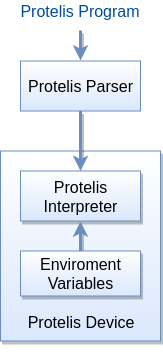
\includegraphics[height=6.8cm]{images/protelis-architecture.png}
    \label{fig:architettura-protelis}
  }\hfill
  \subfloat[Estendibilità di Protelis]{
    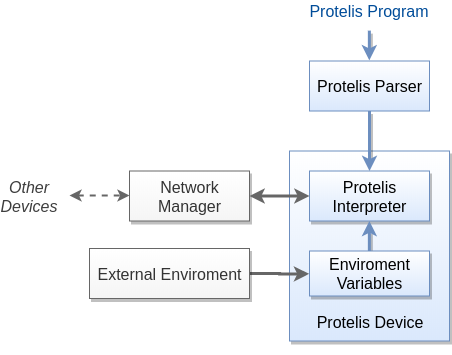
\includegraphics[height=6.8cm]{images/extend-protelis.png}
    \label{fig:estensione-protelis}
  }
  \caption{Architettura astratta di Protelis (a) e meccanismo di estendibilità
    previsto dal linguaggio (b). Immagini tratte da \cite{Protelis}.}
\end{figure}

Protelis è un linguaggio di programmazione aggregato, fortemente influenzato da
Proto\cite{Proto}, la cui esecuzione avviene all'interno di una macchina
virtuale\cite{Protelis}.  Inizialmente un parser traduce un programma Protelis
in una rappresentazione comprensibile all'interprete, che può eseguirlo, in
seguito, a intervalli regolari. L'interprete può interagire con l'ambiente
circostante, implementato tramite coppie \textit{(chiave, valore)} (Figura
\ref{fig:architettura-protelis}).

La duplice possibilità di poter eseguire un interprete Protelis in due contesti
diversi, quali sono un ambiente simulato e quello reale, evidenziano la
necessità dell'introduzione di un componente middleware, che gestisca la
comunicazione tra le macchine virtuali in maniera completamente trasparente a
queste ultime (Figura \ref{fig:estensione-protelis}). Sfruttando la
caratteristica del polimorfismo dei linguaggi ad oggetti, questo modello può
essere facilmente specializzato in entrambi i contesti precedentemente citati.

La piattaforma di supporto scelta per l'implementazione è Java, scelta per la
sua portabilità, il meccanismo interno della reflection, e il sempre crescente
numero di dispositivi embedded a basso costo che supportano Java. Un altro
fattore determinante è l'efficienza in termini di costo di risorse che le
implementazioni Java hanno raggiunto, rendendolo competitivo con linguaggi di
basso livello come C o C++.

Protelis è interoperabile con Java, e indirettamente con Kotlin, di conseguenza
può essere integrato con un vastissimo ecosistema di librerie.

\chapter{Architettura riusabile per backend di Protelis}
\section{Piattaforme di simulazione}
L'architettura utilizzata per Protelis si dimostra flessibile, adatta alla
portabilità su diversi sistemi reali\cite{Clark2015} e simulati quali
Alchemist\cite{alchemist} (Figura 3b) e NASA World Wind\cite{Bell2007}.

L'architettura utilizzata per Protelis si dimostra flessibile, adatta alla
portabilità su diverse piattaforme. Per fare ciò è necessario realizzare un
backend che definisca i meccanismi di comunicazione tra i dispositivi e
gestisca l'esecuzione della macchina virtuale Protelis.

% TODO: Descrizione di alchemist migliore
\subsection{Alchemist}
\begin{figure}
  \centering
  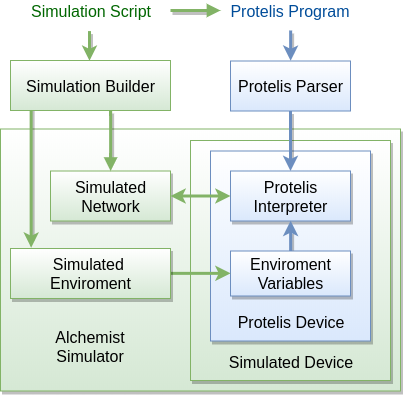
\includegraphics[width=0.7\linewidth]{images/alchemist-architecture.png}
  \caption{Implementazione di Protelis utilizzata in Alchemist.}
\end{figure}
Tra le realizzazioni esistenti l'esempio più rilevante è
Alchemist\footnote{https://alchemistsimulator.github.io/}: un simulatore per
computazione pervasiva, aggregata e ispirata alla natura. Esso utilizza al
proprio interno un meta-modello nel quale dispositivi vicini e interconnessi
comunicano seguendo un insieme di leggi ispirate al mondo della chimica.

Alchemist prevede la probabilità di utilizzare incarnazioni, ovvero
implementazioni concrete del proprio meta-modello per modellare uno specifico
concetto di interesse. Una di queste incarnazioni è quella che consente al
simulatore di eseguire un programma Protelis all'interno della propria
infrastruttura, che permette di creare e gestire una rete di nodi simulati
(Figura /ref{fig:alchemist-architettura}).

\subsection{NASA World Wind}
NASA World Wind\footnote{https://worldwind.arc.nasa.gov/} è un progetto
open-source cross-platform sviluppato dalla NASA, che offre un'interfaccia di
programmazione per creare, in maniera rapida, delle visualizzazioni 3D
interattive di un globo virtuale. Si differenzia da altri software simili come
Google Earth\footnote{https://www.google.it/intl/it/earth/} perché non è una
semplice applicazione, piuttosto un'intera SDK che può essere utilizzata come
base per costruire una propria applicazione.

È stato utilizzato per dimostrare come Protelis possa essere uno strumento che
permette di controllare anche dispositivi reali come uno sciame di droni. In
questa
simulazione\footnote{https://github.com/Protelis/Protelis-Demo-Visualized} 25
quadricotteri, disposti a griglia, volano a qualche centinaio di metri da
terra. Essi fanno uso di comunicazione a corto raggio, 500 metri, per parlare
con i dispositivi adiacenti.

\section{Sistemi distribuiti}

Un sistema distribuito è una collezione di computer indipendenti che appare
all'utente finale come un unico sistema coerente\cite{tanenbaum2016}.  Il
concetto di indipendenza implica che i dispositivi appartenenti al sistema non
abbiano risorse condivise, in particolare la memoria; allo stesso tempo questi
devono tenere un comportamento tra loro armonico. Deve essere quindi prevista
una modalità in cui questi componenti possano comunicare, per scambiarsi
informazioni e coordinarsi.

I costrutti fondanti della programmazione aggregata e i building block possono
semplificare notevolmente il design e lo sviluppo di applicazioni in un contesto
di Internet-of-Things\cite{DBLP:journals/computer/BealPV15}. Essa infatti
consente di costruire, tramite composizione delle proprie API, delle
applicazioni distribuite robuste e affidabili.

Al fine di eseguire macchine virtuali Protelis in un contesto distribuito è
necessario implementare un modello di scambio di messaggi tra queste (Figura
\ref{fig:distributed-deployment}).  L'architettura di Protelis (Sezione
\ref{subsec:Architettura di Protelis}) è stata ideata avendo questo problema ben
chiaro, pertanto è possibile estenderla facilmente, tramite l'implementazione di
uno strato middleware, che si occupi di ciò.


% TODO: API Protelis qui o in architettura?
\section{Architettura riusabile}
\label{sec:model-def}
L'obiettivo di questa sezione è di modellare una architettura del backend di
Protelis abbastanza flessibile, che consenta di incorporare la macchina virtuale
all'interno di un dispositivo, così che attraverso questo sia possibile
eseguirne le iterazioni. Concretamente si effettuerà un mapping delle
caratteristiche di un dispositivo (livello in basso nella Figura
\ref{fig:abstraction-layers}), così che queste possano essere utilizzate per
implementare i costrutti del \textit{field calculus}. Un obiettivo importante di
questo modello sarà circoscrivere in un'entità ben definita il concetto di
strategia di comunicazione. In questo modo il device sarà in grado di funzionare
indipendentemente dal metodo specifico scelto per realizzarla.

% TODO: da scrivere bene un'introduzione
\subsection{API di Protelis}
Le API del backend di Protelis sono scritte in Java, quindi sono facilmente
integrabili anche con linguaggi eseguiti sulla Java Virtual Machine. Esse
offrono le seguenti astrazioni.

\subsubsection{ExecutionContext}
Interfaccia che si pone fra una macchina virtuale Protelis e l'ambiente da cui
essa è circondata. I suoi compiti sono tre:
\begin{itemize}
\item tenere traccia dello stato persistente attraverso le iterazioni successive
  del prorgamma;
\item tenere traccia dell'ultimo stato condiviso dai dispositivi vicini;
\item tenere traccia dell'interazione del dispositivo con l'ambiente esterno
  (tempo, spazio, sensori, attuatori, ecc).
\end{itemize}

\subsubsection{ProtelisVM}
La macchina virtuale Protelis è il nucleo centrale dell'architettura: contiene
l'interprete del linguaggio che al proprio interno implementa gli operatori del
\textit{field calculus}. Accetta in input un \texttt{ProtelisProgram} e utilizza un
\texttt{ExecutionContext} per mantenere il proprio stato e interfacciarsi con
l'esterno. L'interfaccia permette di azionarne i cicli di esecuzione.

\begin{figure}
  \centering
  \includegraphics[width=\linewidth]{diagrams/output/protelis-api}
  \caption{Relazione tra \texttt{ProtelisVM}, \texttt{ExecutionContext} e
      \texttt{ProtelisProgram}.}
  \label{fig:uml-protelisvm}
\end{figure}

\subsubsection{AbstractExecutionContext}
L'interfaccia \texttt{ExecutionContext} contiene la definizione di molti metodi
che dovrebbero essere comuni a tutte le implementazioni di Protelis. Questa
entità astratta realizza quelle procedure delegando a una nuova entità, il
\texttt{NetworkManager}, il compito di stabilire un metodo efficace di
comunicazione.

\subsubsection{NetworkManager}
\label{sec:network-manager}
Astrazione di rete utilizzata dalla macchina virtuale Protelis: ad ogni
iterazione, la macchina virtuale ha bisogno di accedere all'ultimo stato
ricevuto dai vicini e di aggiornare lo stato che verrà inviato ad
essi. L'implementazione di questa interfaccia è cruciale, infatti definisce le
modalità di comunicazione tra i nodi della rete (Figura
\ref{fig:uml-protelisvm}).

Una considerazione importante da fare è che la documentazione ufficiale
specifica che non è necessario che lo stato venga ricevuto o inviato ad ogni
iterazione. La scelta della frequenza di aggiornamento dello stato è demandata
alla specifica implementazione di questa interfaccia, per trovare il rapporto
giusto tra efficienza e condivisione dello stato.

\begin{figure}
  \centering
  \includegraphics[width=\linewidth]{diagrams/output/networkmanager}
    \caption{Introduzione di \texttt{AbstractExecutionContext} e \texttt{NetworkManager}.}
  \label{fig:uml-networkmanager}
\end{figure}

\begin{figure}
  \centering
  \includegraphics[width=\linewidth]{diagrams/output/protelis-vm-sequence}
  \caption{Rappresentazione attraverso un diagramma di sequenza UML di un ciclo
    di esecuzione della macchina virtuale Protelis. Come si vede l'utilizzo di
    diversi \texttt{NetworkManager} specializza il comportamento di tutto il
    sistema.}
    \label{fig:uml-protelisvm-sequence}
\end{figure}


% TODO:
% Serializzazione:
% - time efficient
% - hashing (probabilità molto bassa di errore)
\subsubsection{CodePath}
Rappresenta un percorso, che parte dalla radice dell'albero di esecuzione della
macchina virtuale Protelis e termina in uno dei nodi. Supportando la
serializzazione, viene utilizzato per confrontare l'esecuzione locale a un nodo
con quella dei propri vicini e permettere l'allineamento del codice.

La specifica implementazione di questa classe è critica per la dimensione dei
pacchetti generati dalla comunicazione tra i nodi. Sarà necessario, quindi,
porre l'attenzione su questo aspetto quando la comunicazione sarà basata su
protocolli di rete.

All'interno delle API di Protelis sono già presenti due implementazioni di
questa interfaccia:
\begin{itemize}
\item \texttt{DefaultTimeEfficientCodePath}: il cui algoritmo di generazione è
  orientato alla velocità di esecuzione. L'output non è ottimizzato in termini
  di spazio. Questa implementazione non dovrebbe essere utilizzata quindi per
  l'utilizzo in una rete reale, perché potrebbe generare delle stringhe molto
  lunghe, con conseguenti problemi di performance;
\item \texttt{HashingCodePath}: il cui output dipende dall'algoritmo di hashing
  utilizzato. L'algoritmo di generazione è orientato all'ottimizzazione dello
  spazio, in quanto produce un output di lunghezza predicibile. Quindi è
  l'implementazione consigliata per l'utilizzo in una rete reale. Questa
  versione eredita dall'utilizzo delle funzioni di hashing il rischio di
  collisioni, che diminuisce con l'utilizzo di funzioni più complesse. Spetta al
  progettista la scelta della funzione di hashing che minimizzi le probabilità
  di collisione, massimizzando l'efficienza in termini computazionali.
\end{itemize}

\subsection{Definizione di nuovi concetti}
I concetti che seguono non fanno parte delle API di Protelis, ma sono stati
definiti appositamente per estenderle e creare quindi un nuovo modello, che sia
adatto a rappresentare dispositivi sia in un ambiente reale che in uno simulato.
Questo modello rappresenta dunque una possibile base di partenza per la
realizzazione di un backend di Protelis.

\subsubsection{Capacità di un dispositivo}
\label{sec:device-capabilities}

\begin{figure}
  \centering
  \includegraphics[width=\linewidth]{diagrams/output/device}
  \caption{Introduzione di \texttt{DeviceCapabilities} e \texttt{Device}.}
  \label{fig:uml-device}
\end{figure}

L'obiettivo di questa entità è di realizzare un \texttt{ExecutionContext},
traendo vantaggio delle funzioni già implementate in
\texttt{AbstractExecutionContext}. Implementa le seguenti caratteristiche di un dispositivo:
\begin{itemize}
\item \textbf{Mantenere uno stato nel tempo}: ovvero essere in grado di
  mantenere un insieme di variabili locali e aggiornarle in caso di necessità.
\item \textbf{Comunicare con altri dispositivi}: capacità e protocolli, regole
  utilizzate per effettuare uno scambio di informazioni con altri dispositivi
  vicini. Per fare questo viene riutilizzato il concetto di
  \texttt{NetworkManager} esistente in Protelis.
\item \textbf{Interagire con l'ambiente}: possibilità di interagire con il
  contesto da cui esso è circondato. In un contesto Internet-of-Things, per
  esemio, questo potrebbe concretizzarsi con l'utilizzo di sensori o attuatori.
\item \textbf{Eseguire funzioni definite dall'utente}: facoltà di definire
  funzioni, comportamenti che possono essere richiamate all'occorrente durante
  l'esecuzione del programma.
\end{itemize}

\subsubsection{Device}


Un \texttt{Device} (o dispositivo) è un concetto che rappresenta un singolo
dispositivo in una rete di nodi. Ciascuno di essi incorpora al proprio interno
una macchina virtuale Protelis e sfutta le proprie capacità
(\ref{sec:device-capabilities}), come l'interazione con l'ambiente esterno o la
capacità di mantenere lo stato di una variabile, per supportare l'esecuzione di
quest'ultima.

Un dispositivo per funzionare ha bisogno di un'implementazione concreta di
\texttt{NetworkManager} (\ref{sec:network-manager}), che viene specificata
durante la creazione di uno specifico oggetto, seguendo il pattern strategy. In questo modo il concetto di
dispositivo non è vincolato a uno specifico metodo di comunicazione. Nel
capitolo successivo è presente una dimostrazione della sua riusabilità.

\subsubsection{Speaker}
Implementato sotto forma di strategia funzionale, rappresenta la capacità di un
\texttt{Device} di pubblicare un messaggio, in un modo non definito dall'interfaccia, un
messaggio. Questo verrà gestito e utilizzato in modalità differenti, secondo
la strategia specificata.

La sua implementazione più elementare è \texttt{ConsoleSpeaker}, che prevede che
il messaggio venga stampato sullo standard output.
\begin{figure}
  \centering
  \subfloat[Deployment in simulatore]{
    \includegraphics[width=\linewidth]{diagrams/output/simulation-deployment}
    \label{fig:simulation-deployment}
  }\hfill
  \subfloat[Deployment in ambiente distribuito]{
    \includegraphics[width=\linewidth]{diagrams/output/distributed-deployment}
    \label{fig:distributed-deployment}
  }
  \caption{Rappresentazione attraverso un diagramma UML di deployment delle due
    differenti modalità di comunicazione utilizzate dal \texttt{NetworkManager}
    in contesti distribuiti e simulati. Nella prima i dispositivi appartengono a
    una memoria condivisa, possono usare questa per comunicare. Nella seconda
    ciascun dispositivo appartiene a una diversa Java Virtual Machine, quindi
    devono utilizzare un altro metodo per comunicare, per esempio le socket.}
\end{figure}
\chapter{Esempi applicativi}
In questo capitolo viene provata la flessibilità del modello definito nella
sezione \ref{sec:model-def}, offrendo tre diversi esempi di realizzazione. In
queste dimostrazioni sono presenti numerose assunzioni finalizzate a
semplificare lo sviluppo. Una di queste è che la simulazione inizia quando la
rete ha già effettuato il meccanismo di discovery. Questo consente di fornire a
ciascun dispositivo l'elenco dei propri vicini e concentrare l'attenzione sul
\texttt{NetworkManager}, vero protagonista di questa fase.

Le demo sono state sviluppate sia in Java che in Kotlin,
utilizzando per entrambi un framework di testing, relativamente \textit{Junit} e
\textit{Kotlintest}. In seguito i test sono stati agganciati ad una pipeline di
continuous integration basata su TravisCI\footnote{https://travis-ci.org/}.

Sono stati realizzati un totale di tre esempi applicativi, usando
rispettivamente:
\begin{itemize}
\item un micro-simulatore;
\item un esempio con comunicazione via socket TCP;
\item un esempio con comunicazione via protocollo MQTT.
\end{itemize}

Tutti e tre gli esempi eseguono il medesimo programma aggregato, cambiando solo
la piattaforma di esecuzione. Per ciascun esempio, si fornisce una
implementazione in Java e una in Kotlin. In questo modo si può notare come
l'implementazione del backend sia completamente trasparente al comportamento
finale del sistema. Le simulazioni sono state eseguite su una rete di cinque
dispositivi, disposti secondo topologia ad anello: ciascun dispositivo è quindi
in grado di comunicare solo con quello a sé adiacente.

\begin{minipage}{\linewidth}
\lstinputlisting[caption={Hello, World! in Protelis.},
label=lst:hello-protelis]{code/hello.pt}
\end{minipage}

Il programma Protelis eseguito è un semplice HelloWorld (Listato
\ref{lst:hello-protelis}). Nella prima parte il leader effettua un conteggio a
ritroso. Nella seconda parte i dispositivi adiacenti al leader vengono salutati
da questo.

% Test svolti sempre uguale
%
% Numero di iterazioni
\section{Micro-simulatore}
\begin{figure}
  \centering
  \includegraphics[width=\linewidth]{diagrams/output/emulated-network-classes}
  \caption{Rappresentazione tramite diagramma UML delle classi della classe
    \texttt{EmulatedNetworkManager}. Essa contiente un insieme di
    \texttt{Device} vicini al \texttt{Device} a cui appartiene. Utilizza questi
    riferimenti per inviare loro messaggi.}
  \label{fig:emulated-network-classes}
\end{figure}
\begin{figure}
  \centering
  \includegraphics[width=\linewidth]{diagrams/output/emulated-network-sequence}
  \caption{Rappresentazione attraverso un diagramma UML di sequenza l'uso
    dell'entità \texttt{EmulatedNetworkManager}.}
    \label{fig:emulated-network-sequence}
\end{figure}
La prima implementazione che è stata realizzata è un simulatore.
L'implementazione di Protelis già esistente in Alchemist, quella che utilizza
la libreria NASA World Wind, e quella già esistente nel vecchio repository di
Protelis sono state la linea guida per lo sviluppo di questa versione, in
quanto le strategie di comunicazione sono pressoché le stesse.

In questa modalità i \texttt{Device} sono semplici oggetti eseguiti all'interno
della stessa Java Virtual Machine (Figura \ref{fig:simulation-deployment}). Ne
segue che ciascuno ha visibilità dell'altro in memoria e la comunicazione
avviene, come di consueto nella programmazione ad oggetti, tramite le chiamate
ai metodi; il contenuto dei messaggi è passato come argomento di questi ultimi.

Nello specifico è stata realizzata la classe \texttt{EmulatedNetworkManager},
che simula il comportamento che il \texttt{NetworkManager} avrebbe in una rete
reale. Ciascun \texttt{EmulatedNetworkManager} contiene una lista di
\texttt{Device} vicini(Figura \ref{fig:emulated-network-classes}). Il meccanismo
utilizzato per l'allineamento del codice in fase di esecuzione prevede lo
scambio di un oggetto di tipo \texttt{Map<CodePath, Object>}.
Questo viene passato attraverso un apposito metodo per ricevere un messaggio
dall'esterno, utilizzato nel momento in cui ad un dispositivo viene richiesto di
scambiare lo stato con altri dispositivi (Figura
\ref{fig:emulated-network-sequence}).
L'implementazione del \texttt{CodePath} scelta per questa versione è
\texttt{DefaultTimeEfficientCodePath}, in quanto la dimensione di questo oggetto
non è rilevante, poiché questo viene semplicemente referenziato in memoria,
senza necessità di effettuarne copie.

\section{Comunicazione via socket TCP}
\begin{figure}
  \centering
  \includegraphics[width=\linewidth]{diagrams/output/socket-network-classes}
  \caption{Rappresentazione tramite diagramma UML delle classi dell'entità
    \texttt{SocketNetworkManager}.}
  \label{fig:socket-network-classes}
\end{figure}
\begin{figure}
  \centering
  \includegraphics[width=\linewidth]{diagrams/output/socket-network-sequence}
  \caption{Rappresentazione tramite diagramma UML di sequenza del comportamento
    della classe \texttt{SocketNetworkManager}.}
  \label{fig:socket-network-sequence}
\end{figure}
Questa versione realizza una versione distribuita del backend di Protelis.  È
stata fatta però una semplificazione rispetto a quanto descritto dal diagramma
presente nella Figura \ref{fig:distributed-deployment}): i \texttt{Device} non
sono eseguiti in macchine virtuali Java distinte. Per simulare il fatto che lo
siano essi non possono accedere a zone di memoria condivise. Per comunicare è
necessario che essi utilizzino metodi alternativi, per esempio che utilizzino la
rete IP come tramite.

In questo esempio il passaggio dell'oggetto \texttt{Map<CodePath, Object>}
avviene tramite l'utilizzo di socket TCP. Il protocollo TCP\cite{Postel1981} è
un protocollo di rete di livello trasporto, connesso, che utilizza
un'architettura client-server e che garantisce un canale affidabile di
comunicazione tra due applicazioni su host distinti. La comunicazione avviene
nel seguente modo: un server si mette in ascolto su una determinata porta; un
client invia al server una richiesta di connessione su quella porta. A questo
punto il server accetta la connessione e viene stabilito un canale di
comunicazione affidabile, che può essere utilizzato per lo scambio in entrambe
le direzioni di flussi di dati. La connessione può essere terminata in qualsiasi
momento da uno degli host.

La classe che utilizza le socket è denominata \texttt{SocketNetworkManager}. In
questa versione ciascun \texttt{SocketNetworkManager} contiene al proprio
interno una lista di tuple nella forma \textit{(hostname, porta)}, che
rappresentano i vicini del dispositivo che lo contiene. Ciascuno di essi svolge
un duplice compito di server e client: il primo consiste nel rimanere in ascolto
di connessioni entranti per ricevere messaggi; il secondo comporta stabilire
connessioni con altri \texttt{SocketNetworkManager} quando deve inviare un
messaggio. Una volta che la connessione è stabilita il mittente invia l'oggetto
\texttt{Map<CodePath, Object>} al destinatario, che poi procede a memorizzarlo.

Per permettere il passaggio di un oggetto tramite un protocollo di rete è
necessario effettuarne una serializzazione, ovvero una conversione del suo stato
in una serie di byte, cosicché questa possa essere memorizzata o, in questo
caso, trasferita tramite la rete sotto forma di stream di dati. Una volta giunta
a destinazione questa viene de-serializzata, in modo da poter ricostruire un
oggetto replica dell'originale. I principali metodi utilizzabili per la
serializzazione di oggetti sono: Protocol
Buffers\footnote{https://developers.google.com/protocol-buffers},
JSON\cite{rfc7159}, YAML\cite{ben2009yaml},
Kryo\footnote{https://github.com/EsotericSoftware/kryo},
Elsa\footnote{https://github.com/jankotek/elsa}, etc.. In questa demo, per
motivi di semplificazione, è stata utilizzato il meccanismo di serializzazione
già presente in Java: l'interfaccia \texttt{Serializable}, che, in quanto non
sono presenti particolari richieste in termini di spazio o tempo, soddisfa
pienamente le necessità del progetto.

L'implementazione di \texttt{CodePath} utilizzata in questa demo è
\texttt{HashingCodePath}, in quanto l'oggetto necessita di essere serializzato e
trasferito successivamente tramite la rete. È conveniente dunque che la
dimensione finale di questo sia predicibile a priori.

\section{Protocolli orientati all'Internet-of-Things}
Come già ampiamente discusso, le caratteristiche della programmazione aggregata
la rendono adatta a scenari tipici di ambiti come IoT e reti di sensori. È
importante che l'architettura definita possa supportare le tecnologie e i
protocolli utilizzati in questi ambiti, come MQTT\cite{shinde2016mqtt},
Stomp\footnote{https://stomp.github.io/},
CoAP\cite{rfc7252}, eccetera. In questa sezione viene mostrata
un'implementazione \texttt{NetworkManager} che sfrutta il protocollo MQTT, per
permettere al proprio dispositivo di comunicare con gli altri nodi della rete.

Il protocollo MQTT è un protocollo nato per l'utilizzo nell'ambito
Internet-of-Things e comunicazione \textit{machine-to-machine}. Utilizza il
modello \textit{publish/subscribe}. Questo prevede la presenza di un broker di
messaggistica, un nodo centrale attraverso il quale i client possono registrarsi
per essere notificati di determinati \textit{topic} (argomenti). In qualsiasi
momento un nodo può registrarsi a un nuovo argomento di interesse o inviare un
messaggio a uno di questi. Nel momento in cui il broker riceve un nuovo
messaggio relativo ad un argomento, notifica tutti i client che si erano
registrati ad esso in precedenza. Questo approccio consente di disaccoppiare la
produzione del messaggio dalla sua accettazione, rendendo la comunicazione
asincrona.

\begin{figure}
  \centering
  \includegraphics[width=\linewidth]{diagrams/output/mqtt-network-classes}
  \caption{Rappresentazione tramite diagramma UML delle classi dell'entità
    \texttt{MqttNetworkManager}.}
  \label{fig:emulated-network-classes}
\end{figure}

La classe che utilizza questo protocollo si chiama
\texttt{MqttNetworkManager}. Come la classe \texttt{SocketNetworkManager}
descritta in precedenza, anche questa ha una duplice funzione. La prima è quella
di essere a disposizione per ricevere messaggi: questo avviene mediante la
registrazione, presso un broker centrale, relativa ai messaggi destinati a sé
stesso. La seconda è quella di inviare messaggi agli altri nodi. Per fare questo
ciascun \texttt{MqttNetworkManager} contiene al proprio interno una lista di
argomenti a cui inviare messaggi, uno per ogni vicino; nel momento in cui gli
viene richiesto di inviare l'oggetto \texttt{Map<CodePath, Object>} agli altri
nodi esso lo invia, una volta per ogni argomento, dopo opportuna
serializzazione, al broker di messaggistica, che provvederà a diffondere il
messaggio ai rispettivi destinatari.

Anche in questa versione sono state fatte molte delle scelte effettuate per
quella precedente: i \texttt{Device} sono eseguiti all'interno della stessa Java
Virtual Machine, ma si comportano come se non lo fossero; il serializzatore
scelto è quello incluso nelle librerie di Java; l'implementazione di
\texttt{CodePath} utilizzata è \texttt{HashingCodePath} a causa della necessità
di trasferire questo oggetto tramite la rete.

\begin{figure}
  \centering
  \includegraphics[width=\linewidth]{diagrams/output/mqtt-network-sequence}
  \caption{Rappresentazione attraverso un diagramma UML di sequenza dell'uso
    della classe \texttt{MqttNetworkManager}. La fase di trasmissione di un
    messaggio è ripetuta per ogni dispositivo vicino.}
    .\label{fig:emulated-network-sequence}
\end{figure}

\chapter{Conclusioni e lavori futuri}
\section{Conclusioni}
La programmazione aggregata è un approccio promettente alla risoluzione di
numerosi problemi relativi ai sistemi distribuiti moderni come IoT, reti di
sensori, eccetera.

Partendo dalle API esistenti di Protelis, è stato definito un modello riusabile
che consente di eseguire una macchina virtuale Protelis su diverse
infrastrutture, che possono essere reti reali, come nell'Internet-of-Things
oppure simulate (come nel caso di Alchemist). Per fare ciò si è dovuto
introdurre uno strato che si occupasse della comunicazione tra i nodi in maniera
completamente trasparente ad essi, ovvero in modo che se l'implementazione di
questo cambiasse, il comportamento finale del sistema rimarrebbe lo stesso. Quindi, per
isolare il concetto di comunicazione tra dispositivi dalle entità esistenti, si
è fatto uso del concetto già definito dalle API di Protelis di
\texttt{NetworkManager}, che fornisce una maniera molto semplice di realizzare
lo scambio di messaggi.

A verifica della flessibilità del modello proposto, sono stati portati tre
diversi esempi che rappresentano tre diverse realtà in cui il linguaggio
Protelis può essere utilizzato. In particolare, il primo mira a creare una
simulazione di una rete reale i cui nodi eseguono una macchina virtuale
Protelis; il secondo mostra come l'architettura di Protelis possa essere
facilmente estesa ad un sistema distribuito, supportando la comunicazione
attraverso la rete IP; infine il terzo implementa l'uso di uno dei protocolli
più utilizzati in ambito IoT.

Gli elaborati prodotti sono stati integrati come esempi al repository ufficiale
di Protelis\footnote{https://github.com/Protelis/Protelis-Demo} e rappresentano
un possibile punto di partenza per chiunque voglia implementare un nuovo backend
del linguaggio.

\section{Lavori futuri}
Gli elaborati proposti in questa tesi sono facilmente estendibili. Di seguito
vengono elencati alcuni suggerimenti, per evolvere le demo esistenti o per
svilupparne di nuove. Migliorare
la demo è molto facile: è sufficiente fare un
\textit{fork}\footnote{https://help.github.com/en/github/getting-started-with-github/fork-a-repo}
del repository ufficiale della demo di Protelis, effettuare delle modifiche e
proporle al repository originale tramite una
\textit{pull-request}\footnote{https://help.github.com/en/github/collaborating-with-issues-and-pull-requests/about-pull-requests}.

\subsection{Introduzione di nuove capacità}
Il programma eseguito dai nodi in questi esempi è un semplice Hello, World!
seguito da un conteggio a ritroso. Questo perché la sua finalità non è mostrare
le capacità di Protelis di sfruttare le capacità di un dispositivo reale, bensì
di mostrare come esso si possa adattare a tecniche di comunicazione diverse.  Al
fine di ampliare le dimostrazioni esistenti si potrebbe integrare alle capacità
di un dispositivo: la facoltà di interagire con lo spazio che lo circonda, la
possibilità di interagire con il tempo. In questo modo ciascun dispositivo
acquisirebbe la consapevolezza della propria posizione nello spazio-tempo,
garantendo la possibilità di fruire di nuove tipologie di algoritmi, come il
gradiente. Una possibile e affascinante applicazione di questa nuova tipologia
di dispositivi è il controllo di uno sciame di droni. Infatti, garantendo
ciascuno il controllo della propria posizione nel tempo, ma descrivendone il
comportamento in maniera collettiva, è relativamente semplice prevenire
qualsiasi tipo di collisione, fornendo la possibilità di creare comportamenti o
coreografie in maniera efficace \cite{7789463}.  Protelis fornisce supporto per l'impiego delle
funzioni relative allo spazio e al tempo tramite le interfacce
\texttt{SpatiallyEmbeddedDevice} e \texttt{TimeAwareDevice}.

\subsection{Refactoring della build}
L'elaborato prodotto utilizza Gradle\footnote{https://gradle.org/}, uno
strumento di build automation, per la gestione di sei sottoprogetti, che
consente di controllare in maniera centralizzata l'esecuzione di alcune attività
relative ad essi, come l'esecuzione dei test o la produzione della documentazione.

Nella configurazione attuale, in entrambi i linguaggi utilizzati, l'architettura
riusabile modellata nel corso della tesi è definita solo nel sottoprogetto che
descrive il primo scenario di esempio. Per poterne fare uso, gli altri due
sottoprogetti, tramite una funzionalità di Gradle, importano direttamente i file
sorgenti dal primo. Questa configurazione può essere migliorata introducendo un
nuovo sottoprogetto, nel quale possano essere isolate le parti comuni definite
in questa tesi, che possa essere importato da tutti gli altri.


\subsection{Produzione di ulteriori template}
Si è visto che l'architettura prodotta, per mezzo dell'entità
\texttt{NetworkManager}, si presta all'utilizzo di svariate tecniche e
protocolli di comunicazione. Un possibile miglioramento può essere
l'implementazione di nuovi \texttt{NetworkManager}, che possano utilizzare
tecniche diverse da quelle già utilizzate. In questo modo il repository
ufficiale verrebbe arricchito di nuovi esempi, che possono essere un punto di
riferimento per chi si approccia al linguaggio. Alcune possibili tecniche di
comunicazione che possono essere utilizzate sono:
\begin{itemize}
\item \textbf{STOMP} (Simple Text-orientated Messaging Protocol): protocollo che
  mira ad offrire un canale di comunicazione basato su messaggi di testo, molto
  leggibile per l'uomo, meno efficiente in termini di banda.
\item \textbf{COaP} (Constrained Application Protocol)\cite{rfc7252}: protocollo sviluppato
  per l'interazione tra macchine. Si basa su un model REST, esattamente come
  HTTP, per offrire i propri servizi. È molto competitivo in ambito
  Internet-of-Things a causa della sua capacità di essere eseguito anche in
  dispositivi con pochissime risorse.
\item \textbf{HTTP} (HyperText Transfer Protocol)\cite{rfc7540}: protocollo destinato allo
  scambio di informazioni, come ipertesto, risorse in file di testo o streaming
  video.
\end{itemize}

\subsection{Protelis su dispositivi mobili}
Protelis si basa sull'infrastruttura esistente di Java, infatti viene eseguito
all'interno di una Java Virtual Machine. Questa sua caratteristica può essere
sfruttata per l'implementazione di una versione di Protelis in grado di essere
eseguita all'interno di un dispositivo Android. Infatti le applicazioni per
questi dispositivi sono scritte nativamente in Java e Kotlin, due linguaggi con
cui le API di Protelis si possono interfacciare molto semplicemente. Inoltre la
i sensori presenti in un dispositivo mobile, come uno
smartphone, allargano notevolmente il panorama delle possibili applicazioni.
% \subsection{Ubiquitous computing}
% Ubiquitous computing o ubicomp è un concetto dell'ingegneria del software che si
% contrappone al tipico uso desktop del computer: mentre con questo l'utente deve
% cercare un interazione con un dispositivo come un personal computer, uno
% smartphone, un tablet o un oggetto smart generico, nell'ubicomp l'utente è
% circondato dalla computazione, che avviene in ogni momento e ovunque. Essa può
% avvenire, per esempio, all'interno di un paio di occhiali. La finalità di questa
% è di supportare l'utente nelle sue scelte, nei suoi compiti quotidiani, senza
% che questo lo richieda direttamente. L'Internet-of-Things è una specializzazione
% di questo campo in cui l'interazione è focalizzata tra dispositivi.
%
% La programmazione aggregata, che fornisce costrutti affidabili e robusti per
% realizzare in maniera semplice applicazioni distribuite, è una delle possibili
% tecniche per realizzare questo tipo di sistemi.

% supporto per sistemi ibridi reale-simulato ubicomp

% \input{thesis-parts/acknowledgements.tex}

\backmatter

\bibliography{bibliografia.bib}{}
\bibliographystyle{plain}

\end{document}